\documentclass[13pt,a4paper]{article}

\usepackage[utf8]{inputenc}
\usepackage{graphicx}
\usepackage{wrapfig}
\usepackage{color}
\usepackage{xcolor}
\usepackage{amsmath}
\usepackage{amssymb}
\usepackage[inkscapelatex=false]{svg}
\usepackage{array, makecell}
\usepackage{mhchem}
\usepackage{tabularx}
\usepackage{svg}
\usepackage{braket}
\usepackage{listings}
\definecolor{commentsColor}{rgb}{0.497495, 0.497587, 0.497464}
\definecolor{keywordsColor}{rgb}{0.000000, 0.000000, 0.635294}
\definecolor{stringColor}{rgb}{0.558215, 0.000000, 0.135316}
\lstset{
    frame=single,
    language=Python,
    basicstyle=\ttfamily\vspace{1em},
}

\usepackage[T1]{fontenc}
\usepackage[utf8]{inputenc}
\usepackage[lf]{Baskervaldx} % lining figures
\usepackage[bigdelims,vvarbb]{newtxmath} % math italic letters from nimbus Roman
\usepackage[cal=boondoxo]{mathalfa} % mathcal from STIX, unslanted a bit
\renewcommand*\oldstylenums[1]{\textosf{#1}}

\usepackage{multicol}
\usepackage{colortbl}
\usepackage[Export]{adjustbox}
\adjustboxset{max size={0.9\linewidth}{0.9\paperheight}}
\usepackage[colorlinks=true,linkcolor=red,citecolor=green]{hyperref}

\textwidth=16cm
\textheight=23cm
\topmargin=-2cm
\oddsidemargin=0cm
\setlength{\parindent}{0em}
\setlength{\parskip}{0.6em}
\setlength{\jot}{12pt}
\renewcommand{\arraystretch}{1.4}
\renewcommand{\theadfont}{\bfseries}
\newcommand{\todo}[1]{\textcolor{red}{TODO: #1}}


\begin{document}
\title{
    \LARGE
    \textbf{SATFD lab 04}
}
\author{
    \large
    Dawid Karpiński, 25.04.2024 r.
}
\date{}
\maketitle

\section{Noisy sine signal}

In this section, a noisy sine wave has been generated and different types of filters have been applied to it. The goal is to compare the working of Finite Impulse Response (FIR) and Infinite Impulse Response (IIR) filters in removing noise from a signal.

\begin{lstlisting}[caption={\textbf{Code snippet for generating the noisy sine wave.}}]
N = 2000
A = 5
f = 40
fs = 1000

dt = 1 / fs
times = dt * np.arange(N)
wave = A * np.sin(2 * np.pi * f * times) + A * 2 * np.random.randn(N)


def power_spectrum(
    *, signal: npt.NDArray, fs: int
) -> Tuple[npt.NDArray, npt.NDArray]:
    spectrum = np.fft.fft(signal)

    spectrum = np.abs(spectrum) ** 2
    spectrum = np.roll(spectrum, spectrum.size // 2)

    freqs = np.fft.fftfreq(signal.size, 1 / fs)
    freqs = np.roll(freqs, freqs.size // 2)

    return freqs, spectrum

freqs, spect = power_spectrum(signal=wave, fs=fs)
\end{lstlisting}

This code generates a sine wave with a frequency of 40 [Hz] and an amplitude of 5, sampled at a rate of 1000 [Hz]. The sine wave is then corrupted with random noise.

\begin{figure}[ht!]
    \centering
    \caption{\textbf{Noisy sine wave.}}
    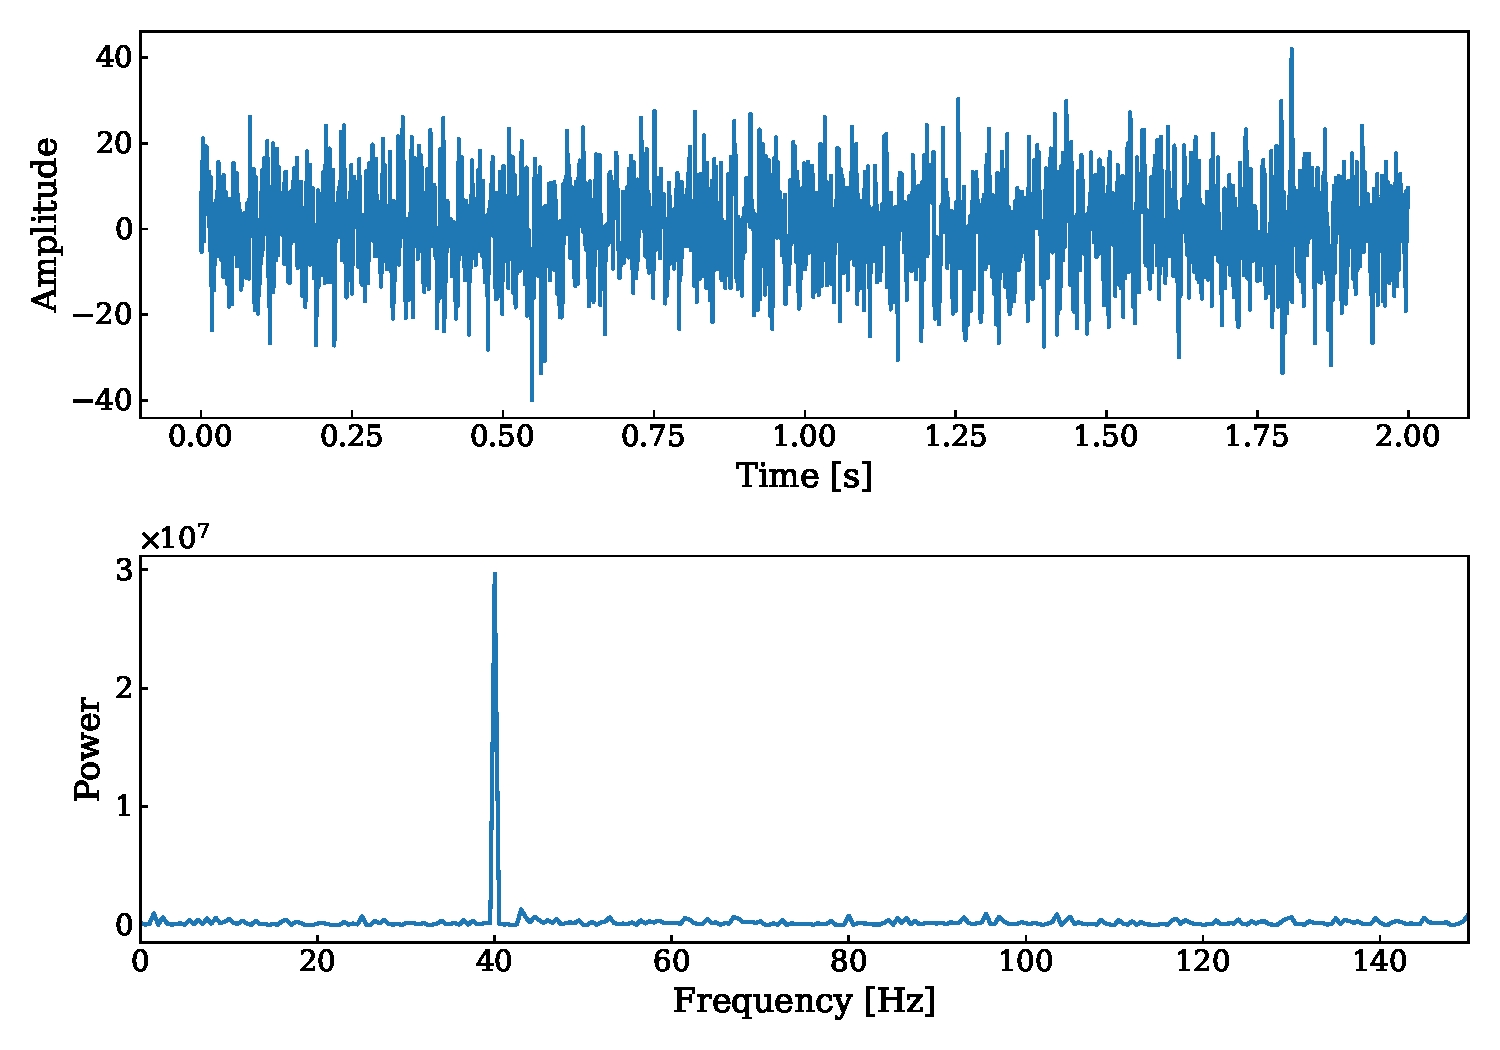
\includegraphics[width=\linewidth]{wave.pdf}
    \label{fig:wave}
\end{figure}
\pagebreak

As can be seen from the figure \ref{fig:wave}, the noise makes it difficult to distinguish the underlying sine wave. In the next sections, different types of filters have been applied to remove the noise and recover the original signal.

Three types of filters have been tested: high-pass, low-pass, and band-pass, for FIR and IIR.

\subsection{FIR filters}

The filters are designed using the \verb|scipy.signal| library, with a filter order of 101. The high-pass filter has a cutoff frequency of 42 [Hz], the low-pass filter has a cutoff frequency of 38 [Hz], and the band-pass filter has a passband of 38-42 [Hz].

The frequency responses are shown in Figures \ref{fig:fir.high-pass}, \ref{fig:fir.low-pass}, and \ref{fig:fir.band-pass}.

\begin{lstlisting}[caption={\textbf{Code snippet for applying the FIR filters.}}]
nyq = fs / 2
order = 101

filters = {
    "highpass": signal.firwin(order, 42 / nyq),
    "lowpass": signal.firwin(order, 38 / nyq, pass_zero=False),
    "bandpass": signal.firwin(
        order, [38 / nyq, 42 / nyq], pass_zero=False
    ),
}

for filter_name, coefs in filters.items():
    fig, [top, mid, bot] = plt.subplots(3, 1)

    result = signal.lfilter(coefs, 1, wave)

    w, h = signal.freqz(b, a, worN=2000)
    top.plot(w * nyq / np.pi, np.abs(h))
    ...
    SNR = 10 * np.log10(signaltonoise(np.abs(result)))
    ...
\end{lstlisting}

\begin{figure}[ht!]
    \centering
    \caption{\textbf{High-pass FIR filter.}}
    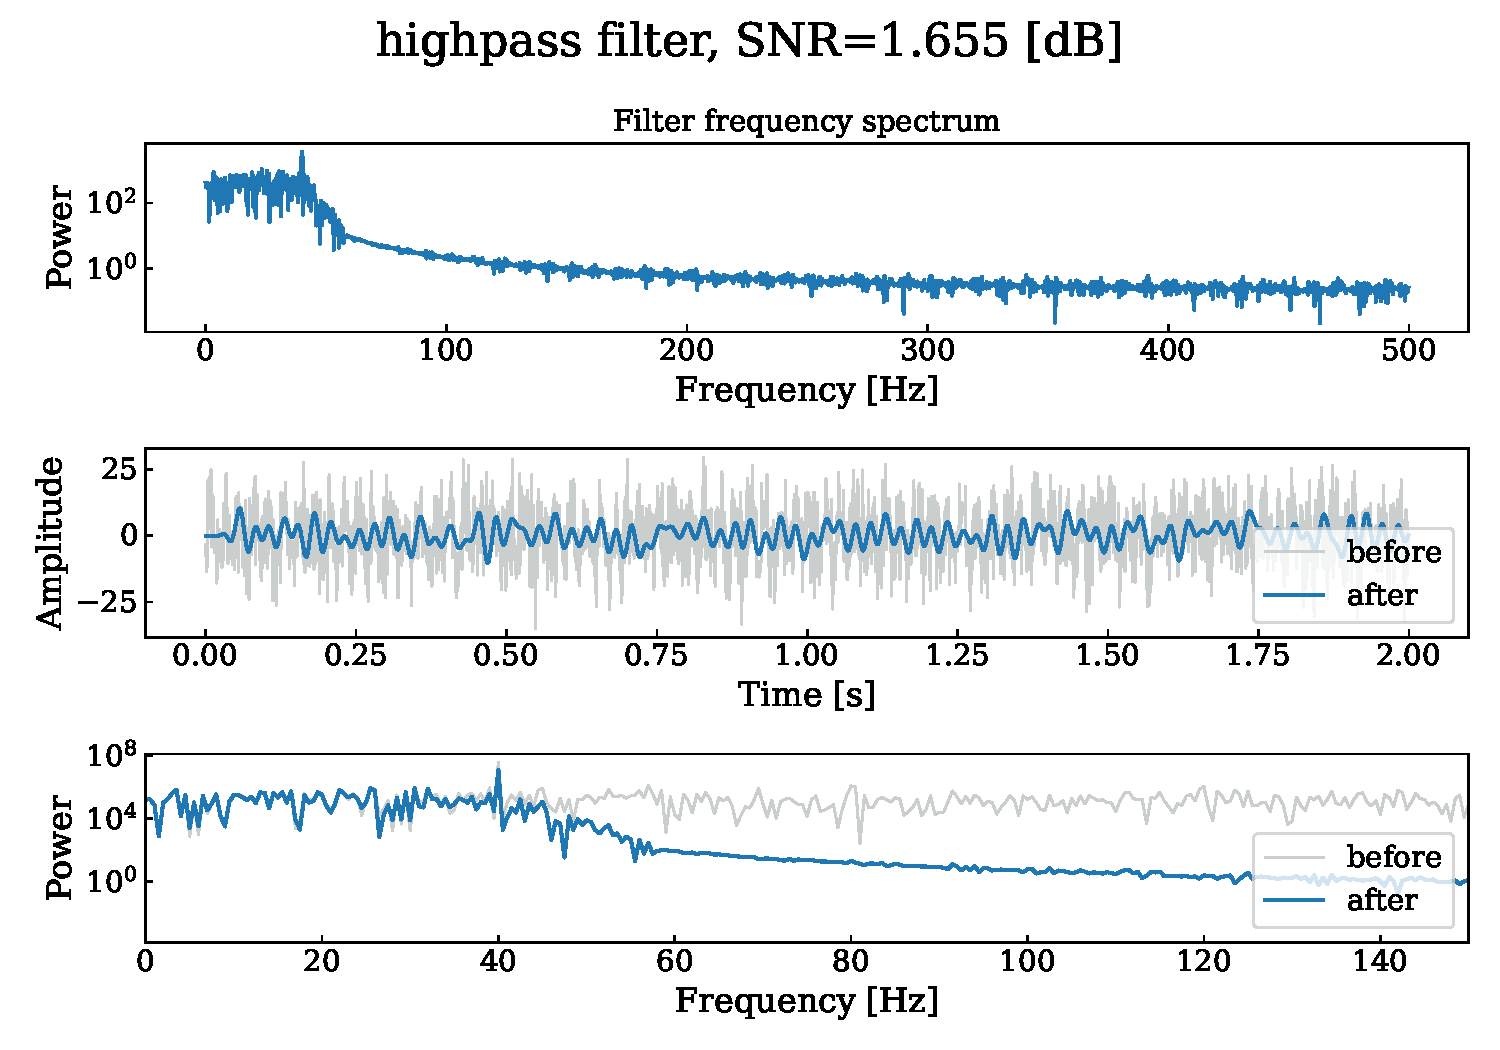
\includegraphics[width=0.9\linewidth]{fir.highpass.pdf}
    \label{fig:fir.high-pass}
\end{figure}

\begin{figure}[ht!]
    \centering
    \caption{\textbf{Low-pass FIR filter.}}
    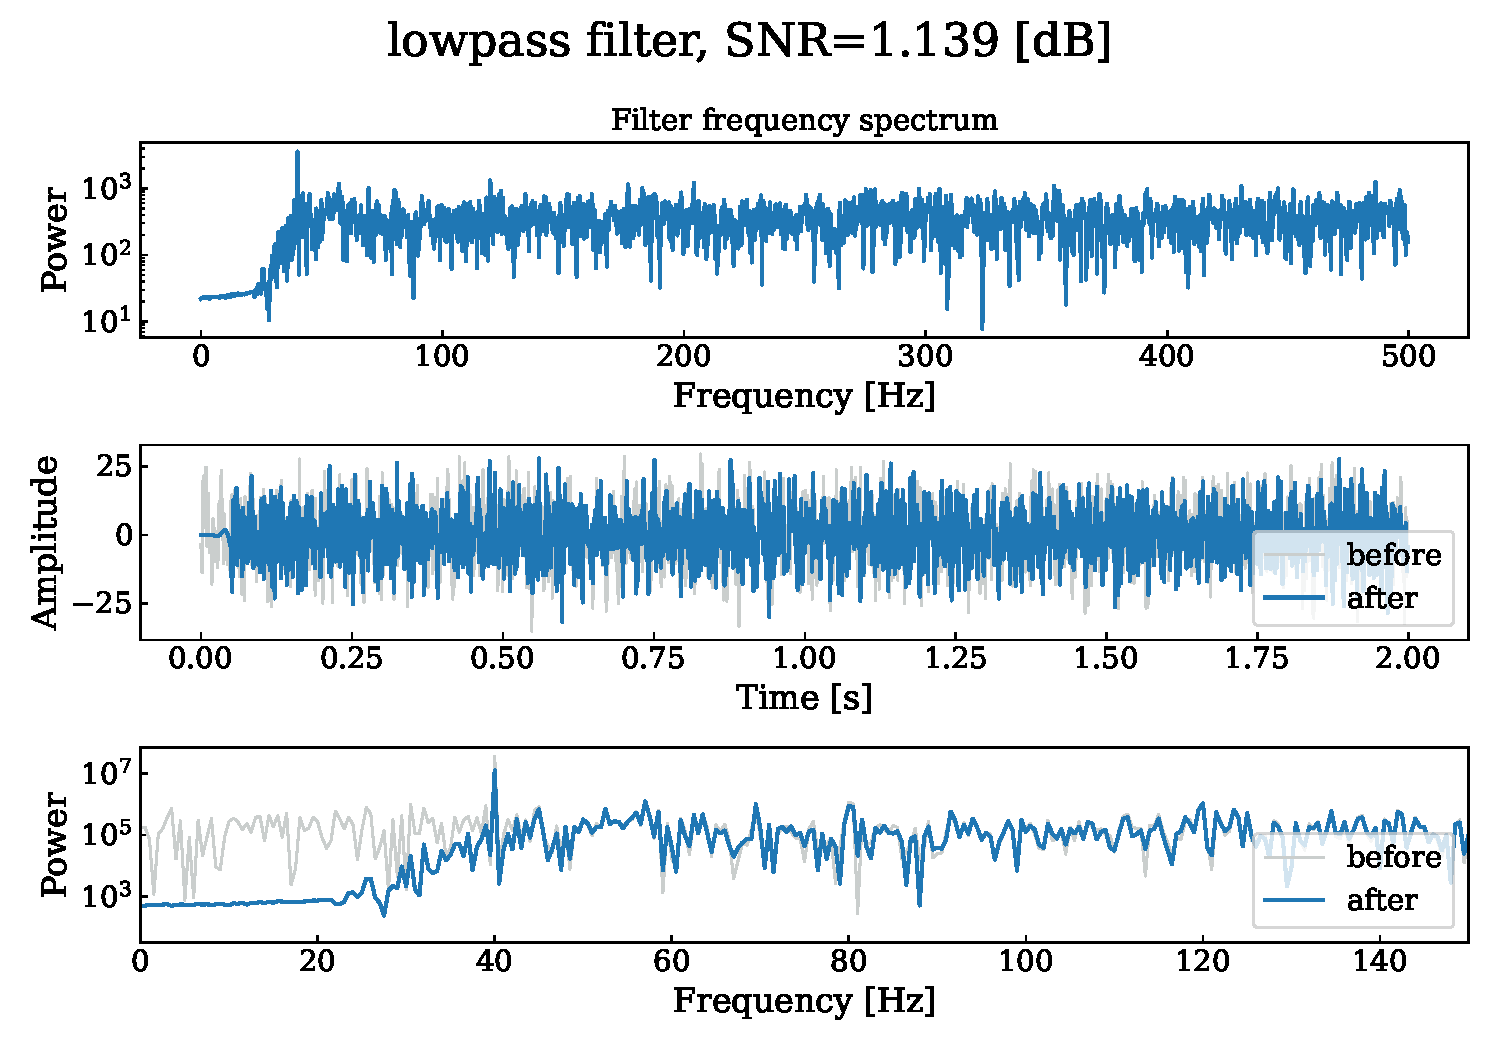
\includegraphics[width=0.9\linewidth]{fir.lowpass.pdf}
    \label{fig:fir.low-pass}
\end{figure}

\begin{figure}[ht!]
    \centering
    \caption{\textbf{Band-pass FIR filter.}}
    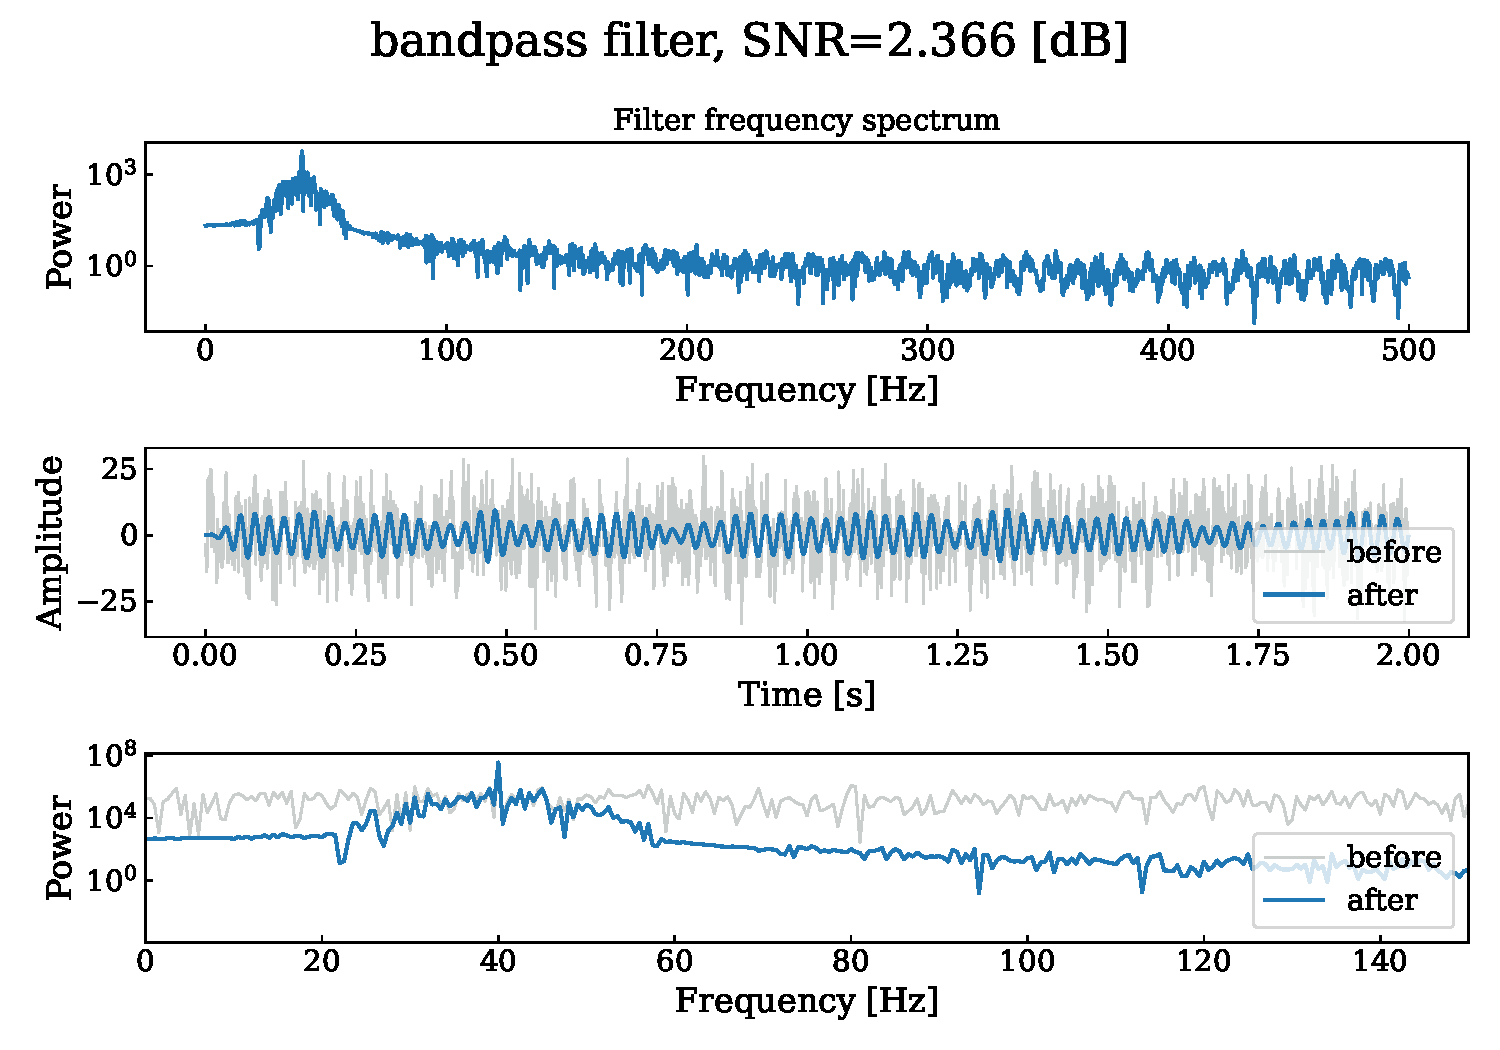
\includegraphics[width=0.9\linewidth]{fir.bandpass.pdf}
    \label{fig:fir.band-pass}
\end{figure}
\pagebreak


\subsection{IIR filters}

The IIR filters have been designed also by using the \verb|scipy.signal| library, with a filter order of 4. Both the high-pass and low-pass filters have a cutoff frequency of 42 [Hz], and the band-pass filter has a passband of 38-42 [Hz].

Their frequency responses are shown in Figures \ref{fig:iir.high-pass}, \ref{fig:iir.low-pass}, and \ref{fig:iir.band-pass}.

\begin{lstlisting}[caption={\textbf{Code snippet for applying the IIR filters.}}]
nyq = fs / 2
order = 4

filters = {
    "highpass": signal.butter(order, 42 / nyq, btype="highpass"),
    "lowpass": signal.butter(order, 42 / nyq, btype="lowpass"),
    "bandpass": signal.butter(
        order, [38 / nyq, 42 / nyq], btype="bandpass"
    ),
}

for filter_name, (b, a) in filters.items():
    fig, [top, mid, bot] = plt.subplots(3, 1)

    result = signal.lfilter(b, a, wave0)

    w, h = signal.freqz(b, a, worN=2000)
    top.plot(w * nyq / np.pi, np.abs(h))
    ...
    SNR = 10 * np.log10(signaltonoise(np.abs(result)))
    ...
\end{lstlisting}

\begin{figure}[ht!]
    \centering
    \caption{\textbf{High-pass IIR filter.}}
    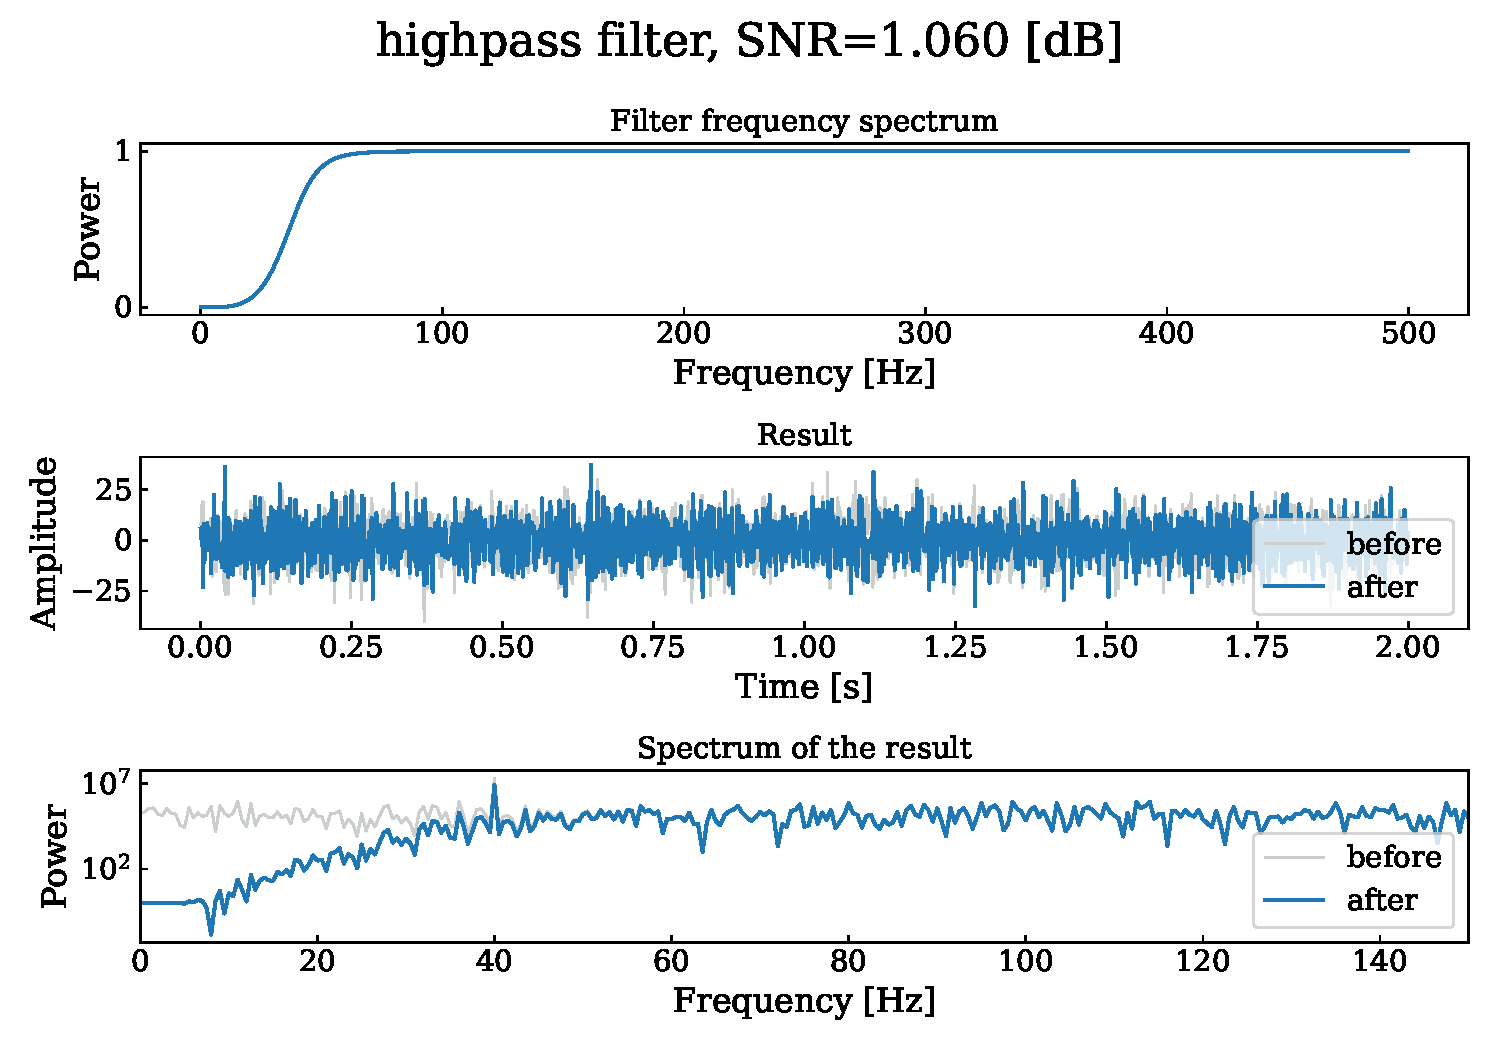
\includegraphics[width=0.9\linewidth]{iir.highpass.pdf}
    \label{fig:iir.high-pass}
\end{figure}

\begin{figure}[ht!]
    \centering
    \caption{\textbf{Low-pass IIR filter.}}
    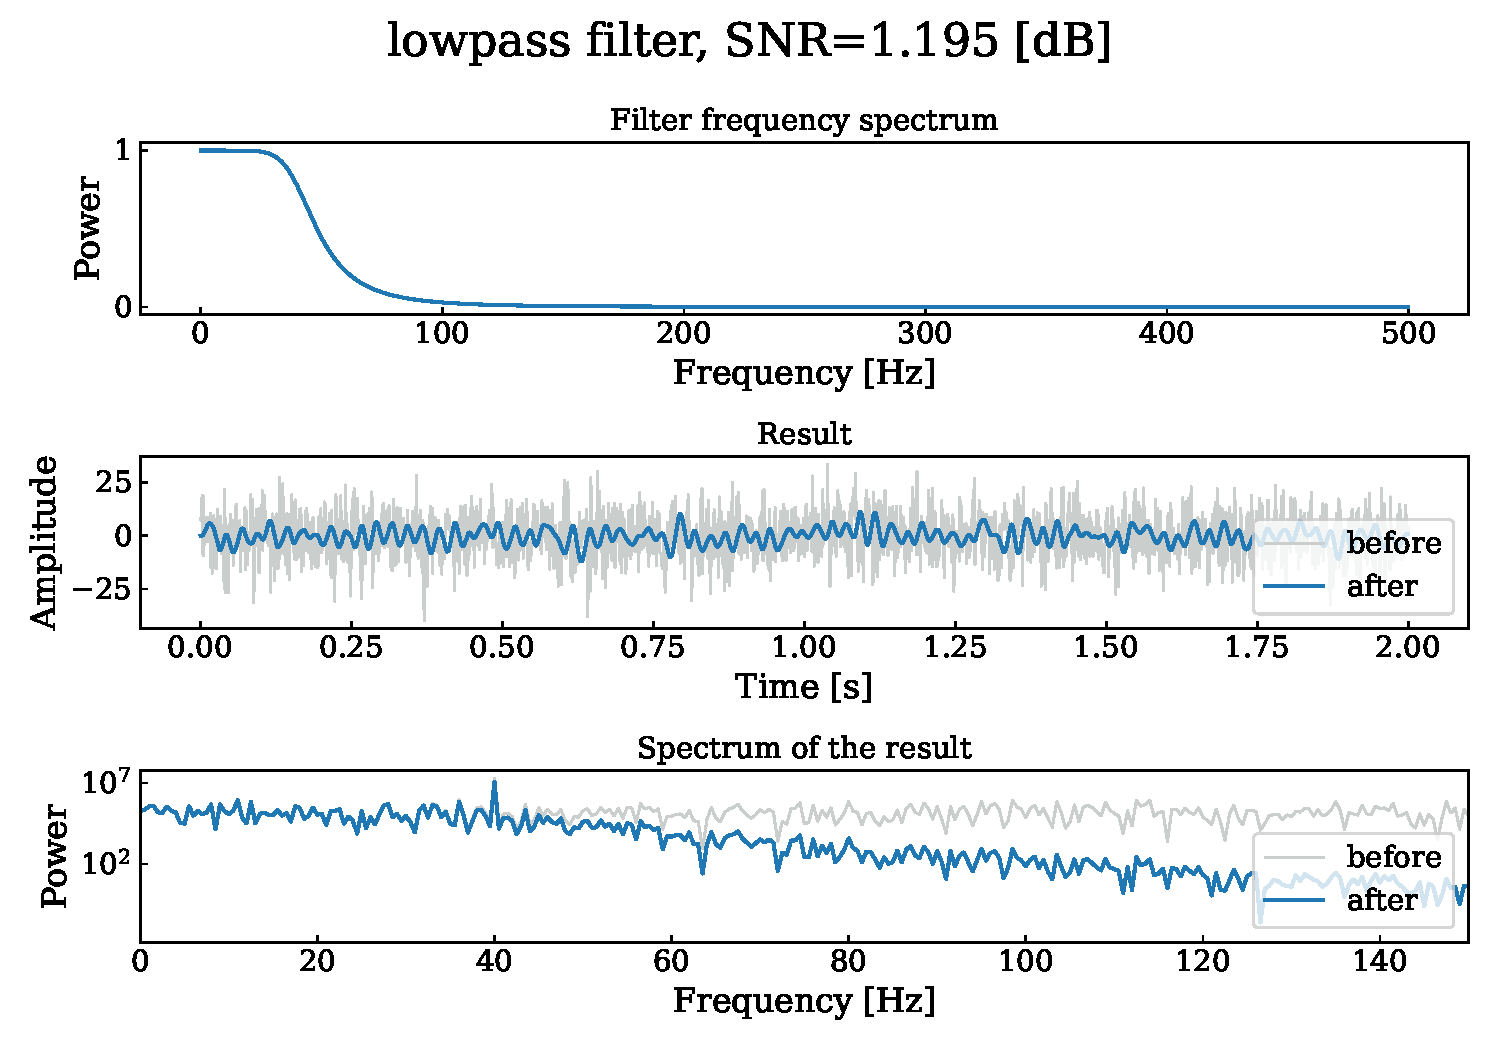
\includegraphics[width=0.9\linewidth]{iir.lowpass.pdf}
    \label{fig:iir.low-pass}
\end{figure}

\begin{figure}[ht!]
    \centering
    \caption{\textbf{Band-pass IIR filter.}}
    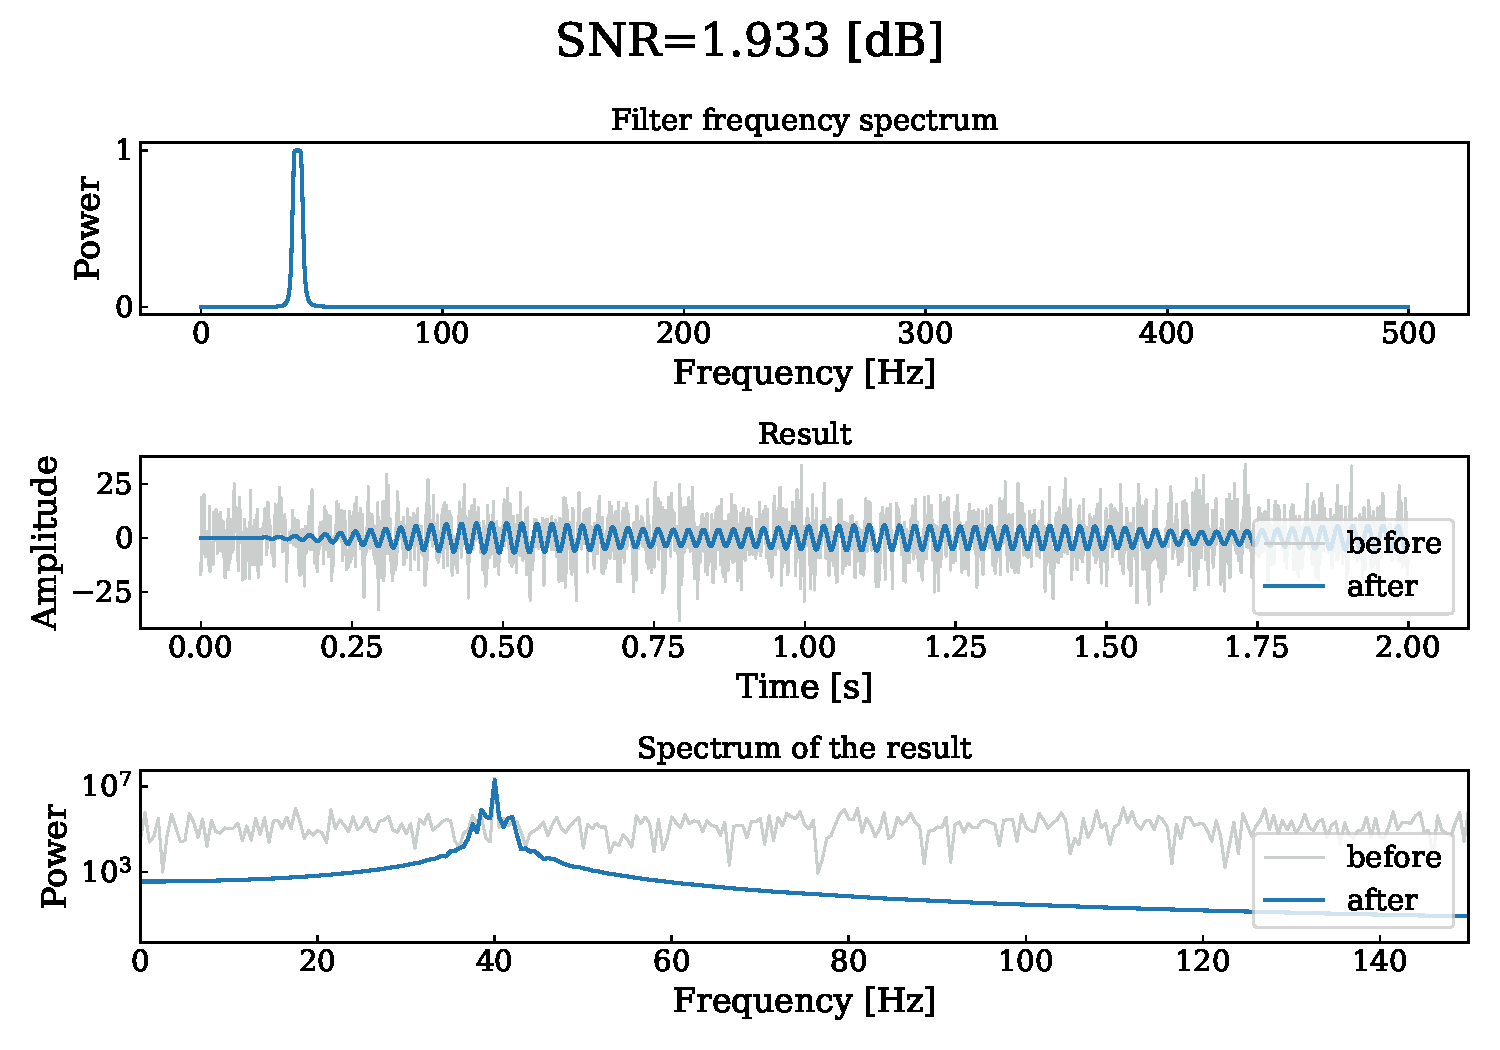
\includegraphics[width=0.9\linewidth]{iir.bandpass.pdf}
    \label{fig:iir.band-pass}
\end{figure}
\pagebreak

As can be seen from the figures, based on the calculated SNR for each filter, the IIR filters are more effective in removing the noise and recovering the original signal.


\section{Two sine waves}

In this section, a sum of two sine waves has been generated. Then, the working of high-pass and low-pass filters have been tested on it. The goal is to demonstrate the ability of these filters to separate two signals with different frequencies.

The sum of two sine waves is generated using the following code:

\begin{lstlisting}[caption={\textbf{Code snippet for generating the two sine waves.}}]
N = 2000
fs = 1000

f1 = 11
f2 = 26
A1 = 2
A2 = 3

times = np.arange(N) / fs
wave = A1 * np.sin(2 * np.pi * f1 * times) + \
       A2 * np.sin(2 * np.pi * f2 * times)

freqs, spect = power_spectrum(signal=wave, fs=fs)
\end{lstlisting}


\begin{figure}[ht!]
    \centering
    \caption{\textbf{Sum of two sine waves.}}
    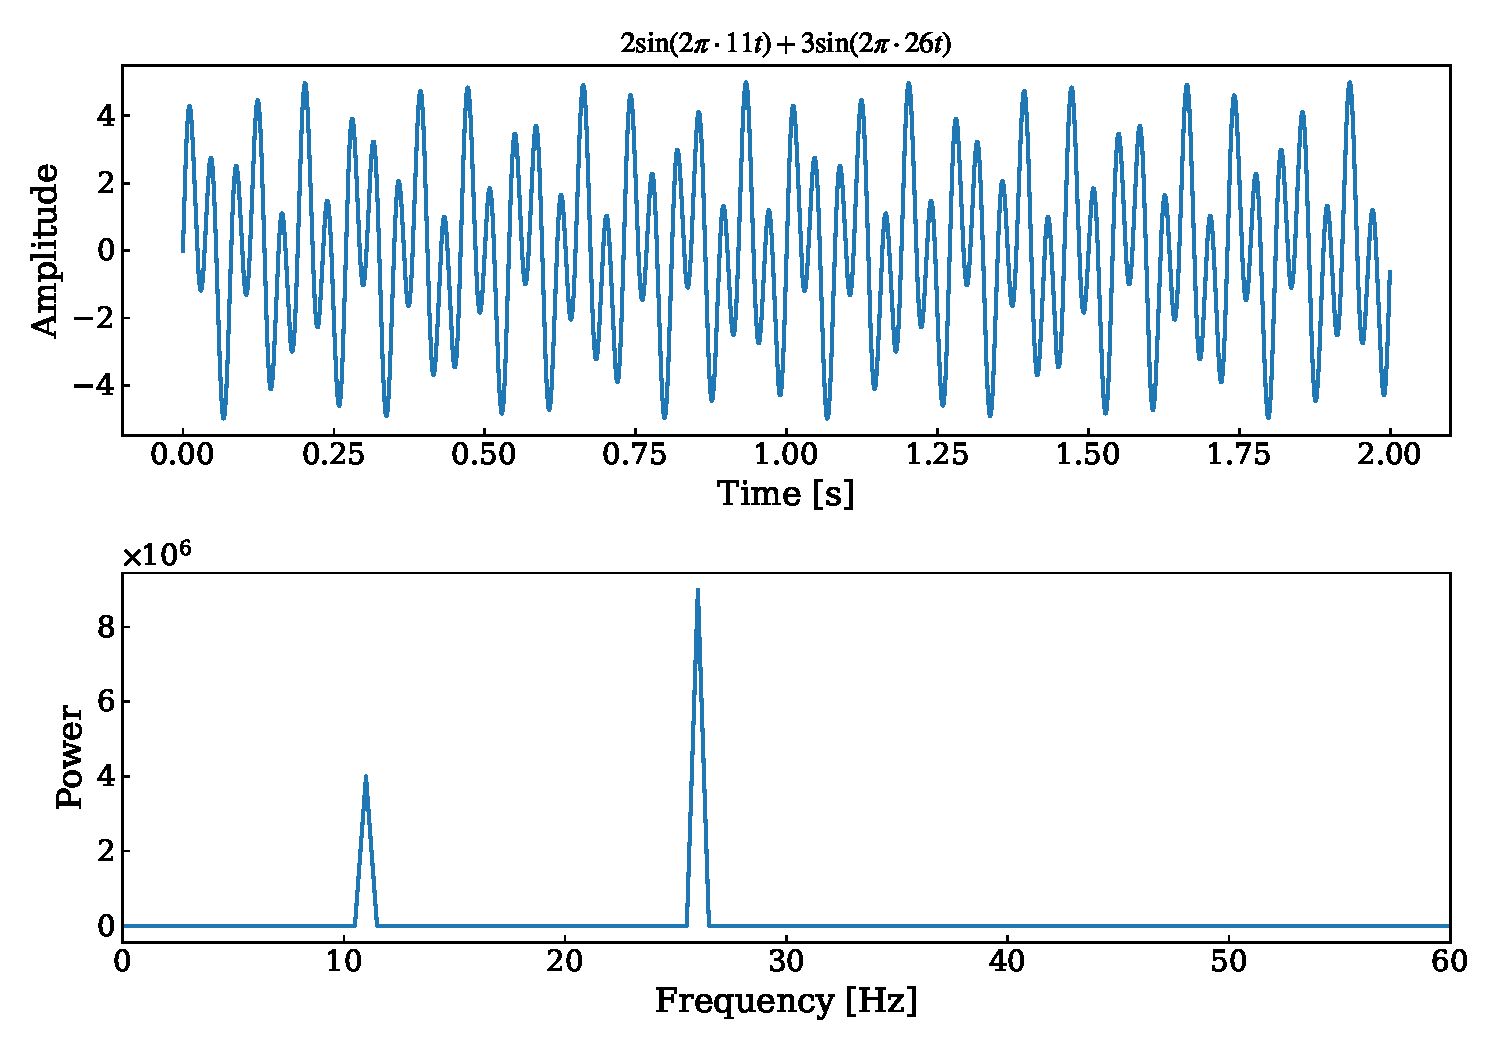
\includegraphics[width=0.9\linewidth]{two_sin.pdf}
\end{figure}

A high-pass filter and a low-pass filter have been applied to the sum of two sine waves, with cutoff frequencies of 1 [Hz] and 36 [Hz], respectively. The frequency responses of these filters are shown in Figures \ref{fig:filter_two_sin.highpass} and \ref{fig:filter_two_sin.lowpass}.

\begin{lstlisting}[caption={\textbf{Code snippet for generating the two sine waves.}}]
nyq = fs / 2
order = 5

filters = {
    "highpass": signal.butter(order, (f1 + 10) / nyq, btype="highpass"),
    "lowpass": signal.butter(order, (f2 - 10) / nyq, btype="lowpass"),
}

for filter_name, (b, a) in filters.items():
    fig, [top, mid, bot] = plt.subplots(3, 1)

    result = signal.lfilter(b, a, wave0)

    w, h = signal.freqz(b, a, worN=2000)
    top.plot(w * nyq / np.pi, np.abs(h))
    ...
    SNR = 10 * np.log10(signaltonoise(np.abs(result)))
    ...
\end{lstlisting}

\begin{figure}[ht!]
    \centering
    \caption{\textbf{Result of high-pass filter on two sines.}}
    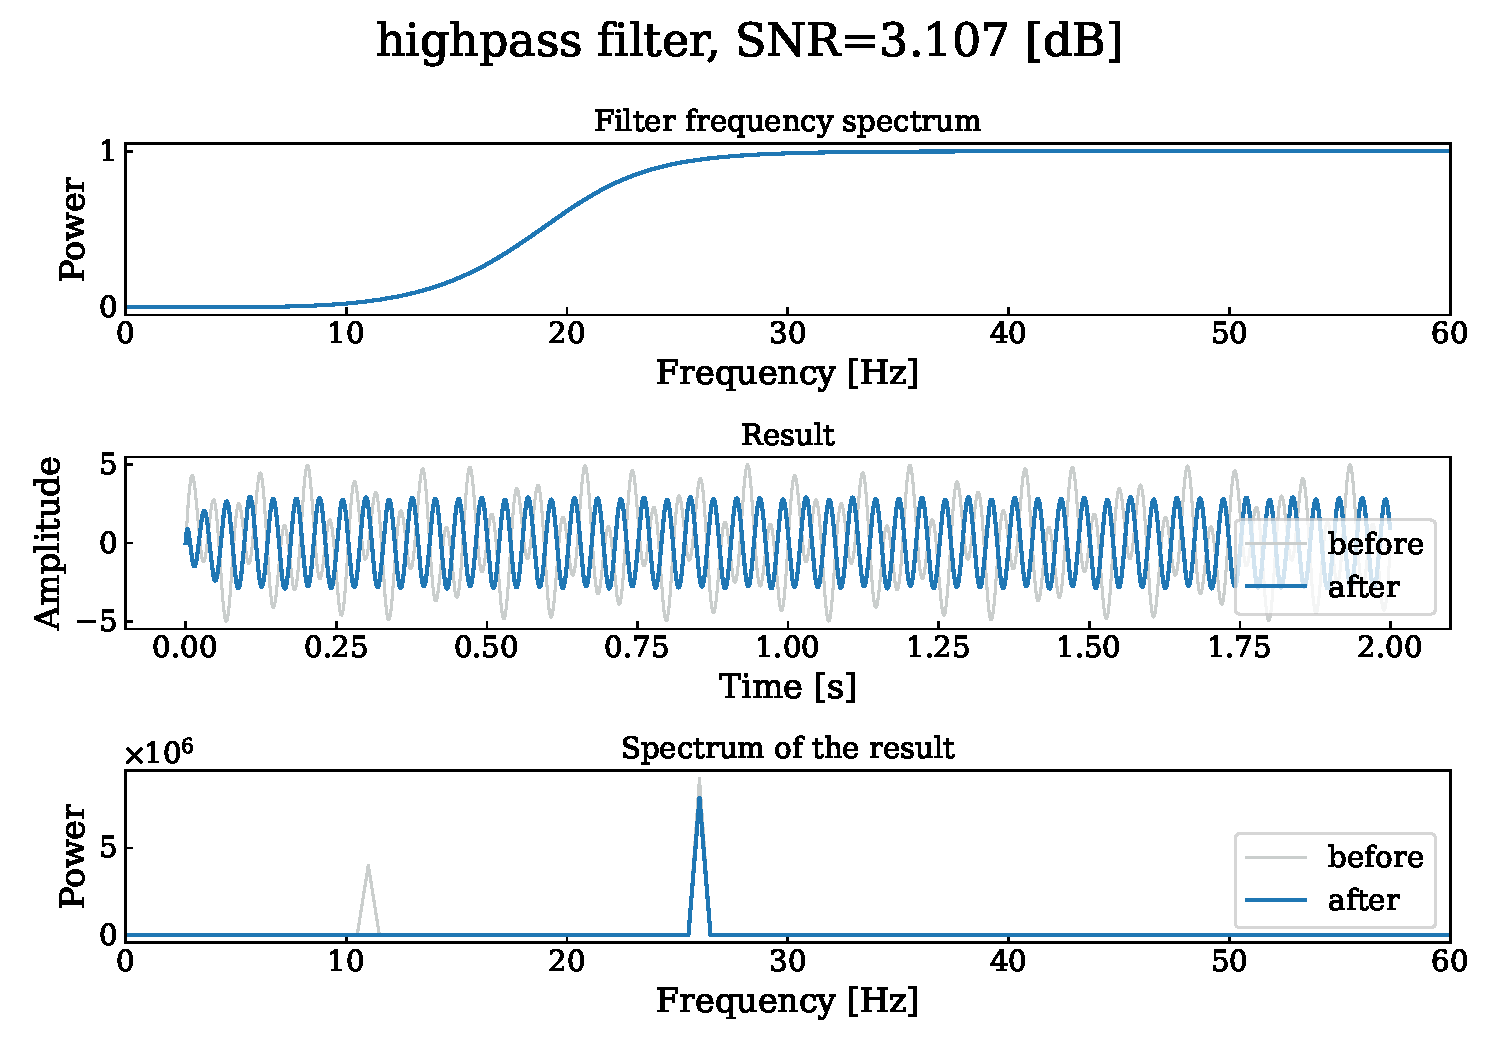
\includegraphics[width=0.9\linewidth]{filter_two_sin.highpass.pdf}
    \label{fig:filter_two_sin.highpass}
\end{figure}

\begin{figure}[ht!]
    \centering
    \caption{\textbf{Result of low-pass filter on two sines.}}
    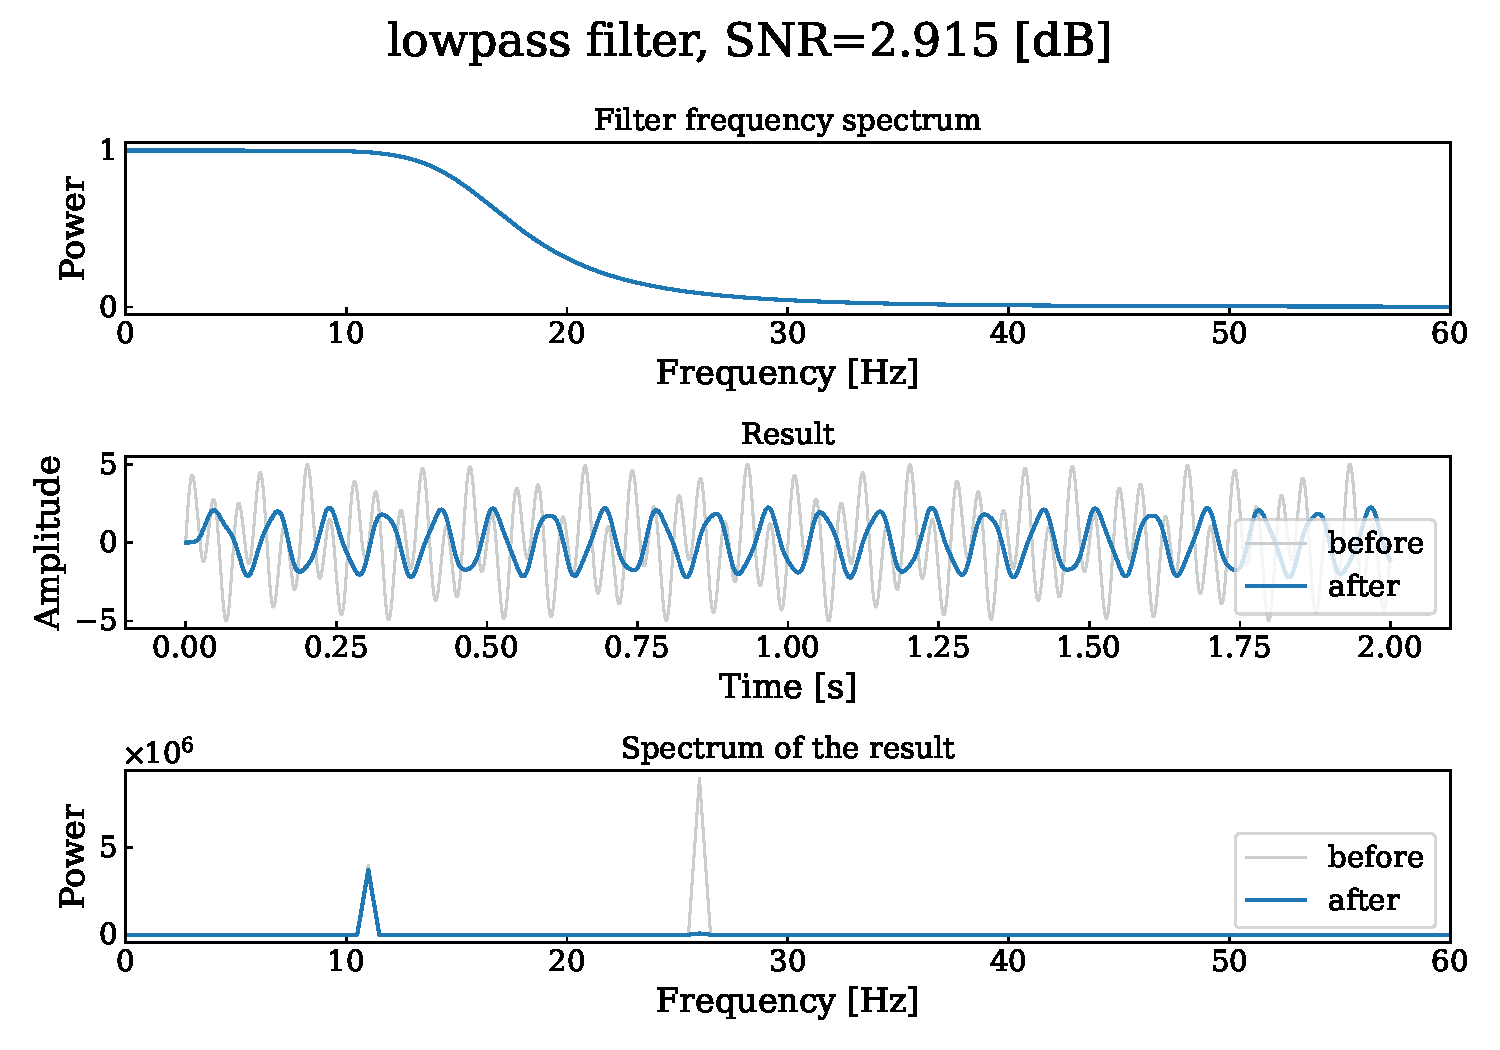
\includegraphics[width=0.9\linewidth]{filter_two_sin.lowpass.pdf}
    \label{fig:filter_two_sin.lowpass}
\end{figure}

As can be seen from the figures, the high-pass filter effectively removes the 11 [Hz] sine wave. The low-pass filter also removes the 26 [Hz] sine wave, however with some distortion left in the resulting signal.

\section{Noisy ECG signal}

In this last section, the filters have been tried on a real-world signal, specifically an electrocardiogram (ECG) signal. The ECG signal is a biomedical signal that measures the electrical activity of the heart. It has been defined by the provided file \verb|ecg.mat|.

To successfully clean the polluted signal, a band-pass filter has been used, with a passband of 0.9-15 [Hz].

\begin{figure}[ht!]
    \centering
    \caption{\textbf{ECG before and after applying the filter.}}
    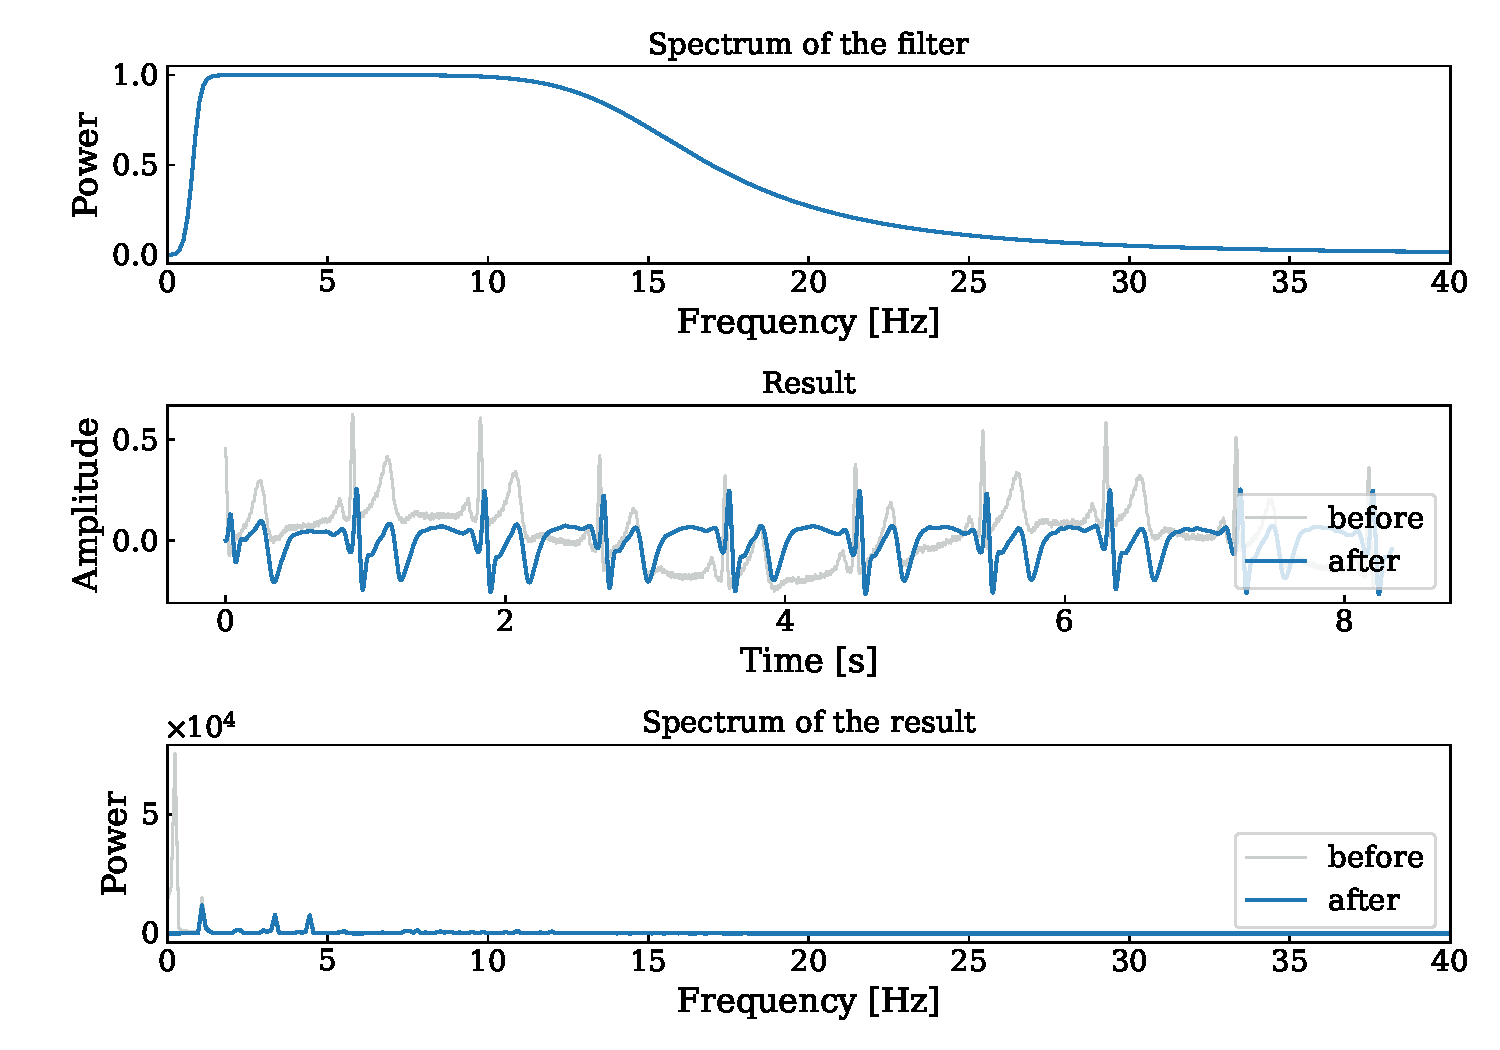
\includegraphics[width=0.9\linewidth]{./ecg_filter.pdf}
    \label{fig:ecg_filter}
\end{figure}

As can be seen from the figure \ref{fig:ecg_filter}, the band-pass filter is enough to largely remove the noise and artifacts from the ECG signal.

\section{Conclusion}

In this report, I have demonstrated the use of FIR and IIR filters to remove noise and artifacts from signals. I have applied these filters to a noisy sine wave, a sum of two sine waves, and a real-world ECG signal. The results show that the filters are effective in removing noise and recovering the original signal.

The entire code for generating the data and plots can be found at:

\url{https://github.com/davkk/signal-analysis/tree/main/sat/lab04}

\end{document}
